\documentclass{standalone}
% pdflatex EnKF_schema.tex
% magick -density 300 EnKF_schema.pdf -quality 90 -resize 640x640 EnKF_schema.png
\usepackage{tikz}
\usetikzlibrary{arrows.meta}
\usepackage{amsmath}
\DeclareMathOperator{\sign}{signo}

\begin{document}

% Models for time series 
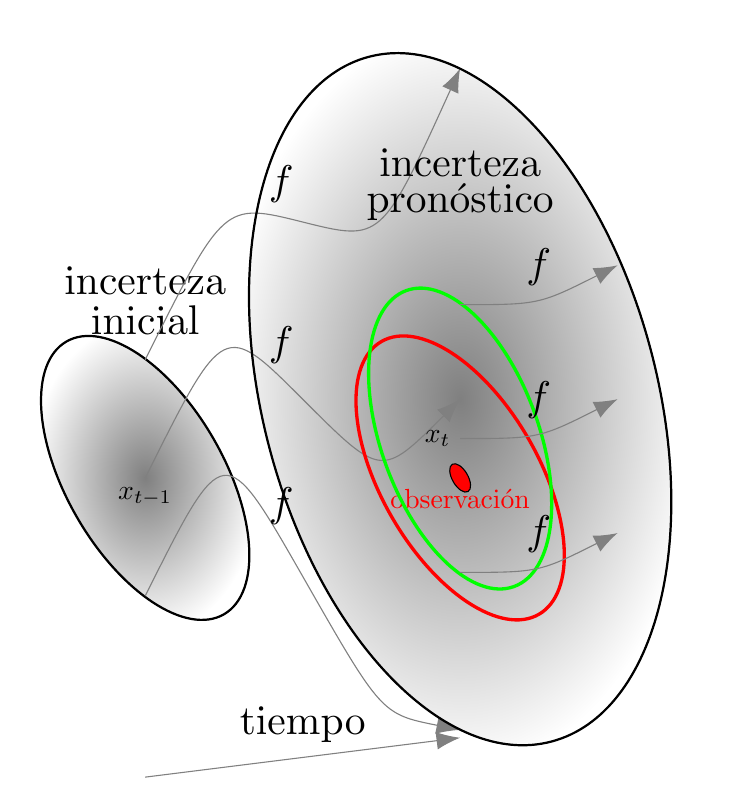
\begin{tikzpicture}


  \shade[inner color=gray, outer color=white, draw=black] (3,3) circle [x radius=1, y radius=2, rotate=30];
    
  \shade[inner color=gray, outer color=white, draw=black] (7,4) circle [x radius=2.5, y radius=4.5, rotate=15];

  \node[below, scale=1] at (3,3) {$x_{t-1}$};
  
  \draw[thick] (3,3) circle [x radius=1, y radius=2, rotate=30];
  \node[scale=1.5, black] at (3,5.5)  {incerteza};
  \node[scale=1.5, black] at (3,5)  {inicial};

  \foreach \x in {-1.5,0,1.5}
  \draw[gray, -{Latex[length=3mm]}] (3,3+\x) .. controls (4,5+\x) .. (5,4+ 1.5*\x)
  node[align=center, above, pos=0.9, scale=1.5, black] {$f$}
  .. controls (6,3+ 2 * \x) .. (7,4+ 2.8 * \x);
  


  \draw[thick] (7,4) circle [x radius=2.5, y radius=4.5, rotate=15];
  \node[scale=1.5, black] at (7,7) {incerteza};
  \node[scale=1.5, black] at (7,6.5) {pronóstico};

  \draw[gray, -{Latex[length=3mm]}] (3,-0.8)  -- (7,-0.3)
  node[align=center, above, pos=0.5, scale=1.5, black] {tiempo};

  \draw[fill=red] (7,3) circle [x radius=0.1, y radius=0.2, rotate=30];
  \draw[draw=red, very thick] (7,3) circle [x radius=1, y radius=2, rotate=30] node[below, scale=1, red] {observación};

  
  \node[below, scale=1, left] at (7,3.5) {$x_t$};
  \draw[draw=green, very thick] (7,3.5) circle [x radius=1, y radius=2, rotate=20];

  \foreach \x in {-1.7,0,1.7}
  \draw[gray, -{Latex[length=3mm]}] (7,3.5 + \x)  ..
  controls (8,3.5 + \x) .. (9,4 + \x)
  node[align=center, above, pos=0.5, scale=1.5, black] {$f$};
  
\end{tikzpicture}


\end{document}
